From the given information, the centre 

\begin{align}
    \vec{c} = \myvec{2\\2} \implies   \vec {u}= -\vec{c} = \myvec{-2\\-2 }
\end{align}

Using the general equation of a circle and substituting $\vec{x} = \myvec{4\\5}$,

\begin{align}
    \label{quadforms/july/2/2/eq:1}
    \begin{split}
\vec{x^\top}\vec{x}+2\vec{u^\top}\vec{x}+f&=0 
\\
\implies     \myvec{4 \ 5}\myvec{4\\5}+\myvec{-4 \ -4}\myvec{4\\5}+f&=0
\\
\implies f+\myvec{41}+\myvec{-36} &= 0 
\\
\text{or, }  f &= -5
    \end{split}
\end{align}
%
Hence , the equation of the circle is,
\begin{align}
    \vec{x^\top}\vec{x}+\myvec{-4 \ -4 }\vec{x}-5=0
\end{align}
%
The radius of the circle is then given by 
\begin{align}
r = \sqrt{\vec{u^\top}\vec{u}-f}
\implies r = \sqrt{13}
\end{align}
%
The above results are verified in Fig.     \ref{quadforms/july/2/2/Figure}


\begin{figure}[!h]
    \centering
    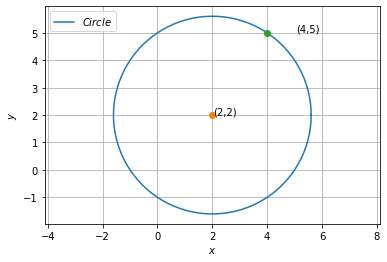
\includegraphics[width=\columnwidth]{solutions/july/2/2/Figures/Figure.png}
    \caption{Plot of the required circle}
    \label{quadforms/july/2/2/Figure}
\end{figure}
